\documentclass{beamer}
\usepackage[utf8]{inputenc}
\usepackage{amsmath, pdfpages, pdflscape, lscape, color, listings, hyperref, amssymb, graphicx,textcomp,varioref, afterpage, subcaption, float, bm, tikz} 

\global
\newcommand{\Fig}[1]{Figure \ref{#1}}
\newcommand{\fig}[1]{figure \ref{#1}}
\newcommand{\tab}[1]{table \ref{#1}}
\newcommand{\eq}[1]{equation \ref{#1}}
\newcommand{\Eq}[1]{Equation \ref{#1}}
\newcommand{\alg}[1]{algorithm \ref{#1}}
\newcommand{\Alg}[1]{Algorithm \ref{#1}}
\newcommand{\chp}[1]{chapter  \ref{#1}}
\newcommand{\Chp}[1]{Chapter  \ref{#1}}
\newcommand{\e}[1]{\cdot 10^{#1}}
\newcommand{\h}{\hbar}
\newcommand{\der}[2]{\frac{\partial #1}{\partial #2}}
\newcommand{\dder}[2]{\frac{\partial^2 #1}{\partial #2^2}}
\newcommand{\p}{\boldsymbol{P}}
\newcommand{\q}{\boldsymbol{q}}
\newcommand{\norm}[1]{\left\lVert#1\right\rVert}
\newcommand{\coef}[2]{\frac{\langle #1,#2\rangle_Q}{\norm{#2}^}}


\newenvironment{test}[1]
{
 \usebackgroundtemplate{}
 \color{gray!30!black}
   \begin{tikzpicture}[remember picture, overlay]
     \node[anchor = center, opacity=.25] (image) at (current page.center) {\includegraphics[scale=0.25]{chaospy_logo.jpg}};
   \end{tikzpicture}
 \begin{frame}[fragile,environment=chaospy]
   
}
{
 \end{frame}
}


\newenvironment{chaospy}[1]
{\color{gray!30!black}
     \color{gray!30!black}
     \usebackgroundtemplate{
   \begin{tikzpicture}[remember picture, overlay]
     \node[anchor = center, opacity=.25] (image) at (current page.center) {\includegraphics[scale=0.25]{chaospy_logo.jpg}};
   \end{tikzpicture}}
     \begin{frame}[fragile,environment=chaospy]
    \frametitle{{#1}}}
{\end{frame}}


\definecolor{keywords}{RGB}{255,0,90}
\definecolor{comments}{RGB}{0,0,113}
\definecolor{red}{RGB}{160,0,0}
\definecolor{green}{RGB}{0,150,0}
 
 
 \lstset{
escapeinside=||
}

 
\usetheme{kalkulo}

\graphicspath{{./figures/}}


\title{Polynomial chaos expansions part I: Method Introduction}
\author{Jonathan Feinberg and Simen Tennøe}


\begin{document}



\begin{frame}
  \maketitle
\end{frame}


\begin{chaospy}{Introduction to Chaospy}
  Chaospy is a Python toolbox specifically developed by yours truly to implement polynomial chaos expansions.\newline
  
  \pause
  \begin{alert}{Task: Install Chaospy by following the instructions}\newline
    
    \href{https://github.com/hplgit/chaospy}{https://github.com/hplgit/chaospy}
    %\newline \href{https://github.com/hplgit/chaospy}{\beamergotobutton{Chaospy}}
  \end{alert}
\end{chaospy}


\section{Introduction}
\begin{frame}
  \frametitle{Introducing the problem}
  We have a simple differential equation
  \begin{align*}
    \frac{d u(x)}{dx} & =-au(x),\qquad u(0) = I,
  \end{align*}
  where $a$ and $I$ are uncertain.\newline
  
    \pause
  Standard notation
  \begin{itemize}
    \item $u(\mathbf{x}, \mathbf{q})$ - Solution to the differential equation.
    \item $\mathbf{q}$ - Parameters with uncertainties, $a$ and $I$.
    \item $D$ - The number of input parameters, $D=2$.
  \end{itemize}
\end{frame}




\begin{frame}
 \frametitle{Introducing the problem}
 The solution for the differential equation is
 \[u(x) = Ie^{-a(x)}\]
 We start by looking at the 1D problem:
 \[a \sim \text{Uniform(0, 0.1)}, \qquad I=1\] 
 The area if interest is 
 \[x=[0,10]\]
%  We also add the complication
%   \[a = \begin{cases}
%         a & t<5\\
%         2a & t \geq 5
%        \end{cases}\]
\end{frame}



\begin{frame}
  \frametitle{Probability space}
  \includegraphics[width=\textwidth]{probspace.png}
\end{frame}



\begin{frame}
 \frametitle{Calculating expectation value analytically}
%  \[E(u) = \int_0^{10}\]
%  \pause
  \begin{align*}
    E(u) &= \int_0^{10}e^{-ax}\frac{1}{10}da\\
%    \uncover<2-> {&= \int_0^{10}e^{-ax}\frac{1}{10}da}\\
    \uncover<2-> {&= -\frac{1}{10x}\left(e^{-10x}-1\right)}\\
    \uncover<3-> { E(u) &= \frac{1-   e^{-10x}}{10x}}\\
 \end{align*}

\end{frame}

\begin{frame}
 \frametitle{Calculating variance analytically}
   \begin{align*}
    Var(u) &= E(u^2) -E(u)^2\\
    \uncover<2-> {&= \int_0^{10}\left(e^{-ax}\right)^2\frac{1}{10}da - \left(\int_0^{10}e^{-ax}\frac{1}{10}da\right)^2}\\
    \uncover<3-> {&= -\frac{1}{20x}\left(e^{-20ax} -1\right) - \left(\frac{1-   e^{-10x}}{10x}\right)^2}\\
   \uncover<4-> {Var(u)&= \frac{1 - e^{-20ax}}{20x} - \left(\frac{1-   e^{-10x}}{10x}\right)^2}
   \end{align*}

\end{frame}

\subsection{Monte Carlo Sampling}

\begin{frame}[fragile]
  \frametitle{One traditional way to solve this problem has been to use Monte Carlo sampling.}
    \begin{figure}
    \includegraphics[width=\textwidth]{MC.png}
  \end{figure}
  \pause
\begin{lstlisting}[language=python]
import chaospy as cp
import numpy as np

def u(x, a):
  return np.exp(-a*x)
    
|\pause|
a = cp.Uniform(0.0.1)
  
\end{lstlisting}
\end{frame}

\begin{chaospy}{Monte Carlo with chaospy}
\begin{lstlisting}[language=python]
samples_a = a.sample(1000)
|\pause|
x = np.linspace(0, 10, 100)
|\pause|
U = [u(x,q) for q in samples_a.T]
U = np.array(U)
|\pause|
E = np.sum(U)/N
Var = np.sum(U**2)/N - E**2
|\pause|
E =  7.15882532019
Var =  2.16180476368
\end{lstlisting}

\end{chaospy}


\begin{frame}
 \frametitle{Error in the approximations}
  \[\varepsilon_E = \int_0^{10}|E(u) - E(\hat{u})|\]
  \[ \varepsilon_{Var} = \int_0^{10}|Var(u) - Var(\hat{u})|\]
 \begin{itemize}
    \item $\varepsilon_X$ - The error in X.
    \item $\hat u$ - approximation of $u$.
  \end{itemize}
\end{frame}


\begin{frame}
  \frametitle{Convergence of Monte Carlo Sampling}
  \begin{figure}
    \includegraphics[width=0.85\textwidth]{MC_convergence_1D_1.png}
  \end{figure}
\end{frame}



\section{Polynomial Chaos}


\begin{frame}
  \frametitle{The general idea behind polynomial chaos expansion}
   \includegraphics[width=0.8\textwidth]{mapping.png}
\end{frame}



\begin{frame}
  \frametitle{Construct polynomial approximation}
  \begin{columns}[c] 
    \column{.5\textwidth}
      Multi-index\\
    \begin{tabular}{c}
    \\
      $\mathbf{P}_{00}$\\
    $\mathbf{P}_{10} \quad \mathbf{P}_{01}$\\
    $\mathbf{P}_{20} \quad \mathbf{P}_{11}\quad \mathbf{P}_{02}$\\
    $\mathbf{P}_{30} \quad \mathbf{P}_{21}\quad \mathbf{P}_{12}\quad ...$ 
  \end{tabular}

\column{.5\textwidth}

Single-index\\
\begin{tabular}{c}
\\
    $\mathbf{P}_{0}$\\
    $\mathbf{P}_{1} \quad \mathbf{P}_{2}$\\
    $\mathbf{P}_{3} \quad \mathbf{P}_{4}\quad \mathbf{P}_{5}$\\
    $\mathbf{P}_{6} \quad \mathbf{P}_{7}\quad \mathbf{P}_{8}\quad ...$ 
  \end{tabular}
  \end{columns}
\end{frame}

\begin{frame}
  \frametitle{Convergence of polynomial approximation}

  \begin{figure}
    \includegraphics[width=0.8\textwidth]{MC_convergence_1D_2.png}
  \end{figure}
  
\end{frame}


\begin{frame}
  \frametitle{Inner product and orthogonality}

    \begin{align*}
    \langle u,v\rangle &= E(u\cdot v)\\
    \uncover<2->{&= \int f_Q(q)u(x,q)v(x,q)dq}
  \end{align*}
  
\begin{itemize}
 \onslide<3->\item $f_q(q)$ - 
\end{itemize}

  \onslide<4->
  Orthogonality
  \[\langle P_n,P_m\rangle =
  \begin{cases}
    \norm{P_n}^2_Q & n = m \\
    0 & n \neq m
  \end{cases}\]

\end{frame}

\begin{frame}
\frametitle{Why is this a good idea?}
\begin{block}{Theorem:}
  \[\norm{u-\hat{u}_M}_Q \leq \norm{u-u^*}_Q \qquad \text{for all } u^* \in \mathbb{P}_M\]
\end{block}

\begin{itemize}
\onslide<2-> \item $\hat{u}_M$ - Orthogonal approximation, of order M
\end{itemize}

\onslide<3->
Assumptions: 
\begin{itemize}
  \item $P_0,...,P_N$ are mutually orthogonal polynomials
  \onslide<4->\item $c_0,...,c_N$ are Fourier coefficients, $c_n = \frac{\langle u, P_n\rangle}{\norm{P_n}^2_Q}$
 \end{itemize}
\onslide<5->
 This also leads to 
  \[\text{Var}(|u-\hat{u}_M|)\leq \text{Var}(|u-u^*|)_Q \qquad \text{for all } u^* \in \mathbb{P}_M\]
\onslide<6->
The number of terms N is give by:
  \[N = \frac{(M+D)!}{(MD)!} -1\]
\end{frame}

\begin{frame}
 \frametitle{When we have constructed $\hat{u}_M$ we also know}
   \begin{align*}
  E(\hat u_M) &= c_0\\
   \uncover<2->{Var(\hat u_M) &= \sum_{n=1}^N c_i^2\norm{\p_n}_{Q}^2}
  \end{align*}
  \onslide<3->
 This leaves us with the following two challenges, finding:
 \begin{itemize}
  \item $P_0,...,P_N$
  \item $c_0,...,c_N$
 \end{itemize}
\end{frame}

\begin{frame}
 \frametitle{Proposal, let us use Gram-Schmidt to find the orthogonal polynomials}
%  Assumption: We are in 1D and have $a +~ F_q$ and $I = 1$. 
 \[V_0, V_1,...,V_N = 1, q,...,q^N\]
 \pause
 The Gram Schmidt method is
 
 \begin{align*}
    P_0 &= V_0\\
    \uncover<3-> {P_n &= V_n - \sum_{m=0}^n \frac{\langle V_n,P_m\rangle_Q}{\norm{P_m}^2_Q}}\\
  \uncover<4-> {&= V_n - \sum_{m=0}^n\frac{\mathbb{E}(V_nP_m)}{\mathbb{E}(P_m^2)}}
 \end{align*}

\end{frame}

\begin{chaospy}{Gram-Schmidt with chaospy}
\begin{lstlisting}[language=python]
M = 5; D = 1
N = factorial(M+D)/factorial(M) - 1
a = cp.Uniform(0,0.1)
|\pause|
V = cp.basis(0,M,1)
P_M = [V[0]]
|\pause|
for n in xrange(1,N):
    summation = 0
    for m in xrange(0,n):
        summation += P_M[m]*cp.E(V[n]*P_M[m],a)
                            /cp.E(P_M[m]**2,a)
    P_M.append(V[n] - summation)
 \end{lstlisting}
\end{chaospy}


\begin{frame}
 \frametitle{Plot of all generated polynomials}
  \begin{figure}
    \includegraphics[width=0.85\textwidth]{gramschmidtpoly.png}
  \end{figure}
\end{frame}


\begin{frame}
 \frametitle{But once again things go wrong}
  %plot the errors as we go to large M
    \begin{figure}
    \includegraphics[width=0.8\textwidth]{gramschmidterror1.png}
  \end{figure}
  
 \end{frame}


\begin{frame}
 \frametitle{The Three Term Recurrence (TTR) relation}
  All orthogonal polynomials satisfy the three term recurrence relation
  \[P_{N+1} = (x-A_n)P_n - B_nP_{n-1}\]
  \[P_{-1} = 0\qquad P_0 =1\]
    \pause
   Where:
  \[A_n = \frac{\langle q,P_n\rangle_Q}{\norm{P_n}}\]
  \[B_n = 
  \begin{cases}
  \frac{\norm{P_n}^2_Q}{\norm{P_{n-1}}} \qquad n > 0\\
  \norm{P_n}^2_Q \qquad n = 0
  \end{cases}
  \]
  \end{frame}

\begin{chaospy}{TTR with chaospy}
\begin{lstlisting}[language=python]
import chaospy as cp

M = 3
a = cp.Normal()
P = cp.orth_ttr(M, a)

print P

[1.0, q0, q0^2-1.0, q0^3-3.0q0]
\end{lstlisting}
\end{chaospy}

\begin{frame}
 \frametitle{Things are better now}
    %plot the errors as we go to large M
    \begin{figure}
    \includegraphics[width=0.8\textwidth]{gramschmidterror2.png}
  \end{figure} 
 \end{frame}
  
\begin{frame}
 \frametitle{The Three Term Recurrence (TTR) relation}
\includegraphics[width=0.9\textwidth]{k_convergence.png}
 \end{frame}


\begin{chaospy}{Finding the Fourier coefficients}
 \begin{lstlisting}[language=python]
def u(x,a):
  ax = np.outer(a,x)
  return np.exp(-ax)
|\pause|
m = 2
a = cp.Uniform(0,0.1)
x = np.linspace(0, 10, 100)
|\pause|
P, norm = cp.orth_ttr(m, a, retall=True)|\pause|
nodes, weights = cp.generate_quadrature(m+1, a,
                                        rule="G")|\pause|
solves = u(x,nodes[0])|\pause|
u_hat, c = cp.fit_quadrature(P, nodes, weights,
                             solves,retall=True)
\end{lstlisting}

\end{chaospy}


\begin{frame}
\frametitle{Convergence of orthogonal polynomial approximation}

  \begin{figure}
    \includegraphics[width=0.8\textwidth]{MC_convergence_1D_3.png}
  \end{figure}
   \end{frame}


\begin{frame}
 \frametitle{Multidimensional problems}
 
 \[a \sim \text{Uniform(0, 0.1)}, \qquad I \sim \text{Uniform(8, 10)}\] 
 \pause
  \begin{align*}
  P_n &= P^{(1)}_n, ..., P^{(D)}_{n_D}
  & n\longleftrightarrow (n_1, ..., n_D)
  \end{align*}
  \pause
  \includegraphics[width=\textwidth]{multidim.png}
   
 % \begin{tabular}{l|cccccc}
 % ... &&&&&\\ 
  % $\mathbf{P}_{4}$& ...&&&& \\
 %   $\mathbf{P}_{3}$ &	$\mathbf{P}_{3}\mathbf{P}_{0}$ & ... && &\\
 %   $\mathbf{P}_{2}$ &	$\mathbf{P}_{2}\mathbf{P}_{0}$ & $\mathbf{P}_{2}\mathbf{P}_{1}$ & ... &&& \\
 %   $\mathbf{P}_{1}$ &	$\mathbf{P}_{1}\mathbf{P}_{0}$ &$\mathbf{P}_{1}\mathbf{P}_{1}$& $\mathbf{P}_{1}\mathbf{P}_{2}$ & ...&&\\
 %   $\mathbf{P}_{0}$ &	$\mathbf{P}_{0}\mathbf{P}_{0}$ &$\mathbf{P}_{0}\mathbf{P}_{1}$& $\mathbf{P}_{0}\mathbf{P}_{2}$ & $\mathbf{P}_{0}\mathbf{P}_{3}$ & ...\\ \hline
%		     &	$\mathbf{P}_{0}$	&$\mathbf{P}_{1}$& $\mathbf{P}_{2}$ & $\mathbf{P}_{3}$ & $\mathbf{P}_{4}$& ...
%  \end{tabular}
 \end{frame}


\begin{frame}
 \frametitle{Multidimensional orthogonality}
\begin{align*}
 \langle P_n, P_m\rangle &= \mathbb{E}(P_{n_1}^{(1)}\cdots P_{n_D}^{(D)}\cdot P_{m_1}^{(1)}\cdots P_{m_D}^{(D)}\\
  \onslide<2-> {&= \mathbb{E}(P_{n_1}^{(1)}\cdot P_{m_1}^{(1)})\cdots \mathbb{E}(P_{n_D}^{(D)}\cdot P_{m_D}^{(D)})} \\
  \onslide<3-> {&= \langle P_{n_1}^{(1)}\cdot P_{m_1}^{(1)} \rangle\cdots  \langle P_{n_D}^{(D)}\cdot P_{m_D}^{(D)} \rangle} \\
  \onslide<4-> {&= \begin{cases}
       0 & n_d \neq m_d \quad \text{There exists a } d \text{ such that }n \neq m\\
      \norm{P}^2 & \text{else} 
     \end{cases}}
\end{align*}

 \end{frame}


 
 \begin{chaospy}{Code example}
\begin{lstlisting}[language=python]
a = cp.Uniform(0, 0.1)
I = cp.Uniform(8, 10)
dist = cp.J(a,I)
|\pause|
P = cp.orth_ttr(1, dist)
print P
[1.0, q1-9.0, q0]
|\pause|
P = cp.orth_ttr(3, dist)
print cp.E(P[1]*P[2],dist)
0.0 |\pause|
print cp.E(P[3]*P[3],dist)
0.0888888888903
\end{lstlisting}
\end{chaospy}
 
 
 \begin{chaospy}{Convergence of a multidimensional problem}
 \begin{lstlisting}[language=python]
def u(x,a, I):
  return I*np.exp(-a*x)
|\pause| 
a = cp.Uniform(0, 0.1); I = cp.Uniform(8, 10)
dist = cp.J(a,I)|\pause|
x = np.linspace(0, 10, 100)
m = 2
|\pause| 
P = cp.orth_ttr(m, dist)|\pause|
nodes, weights = cp.generate_quadrature(m+1, dist,
                                        rule="G")|\pause|
i1,i2 = np.mgrid[:len(weights), :100]|\pause|
solves = u(x[i2],nodes[0][i1],nodes[1][i1])|\pause|
u_hat = cp.fit_quadrature(P, nodes, weights,
                          solves)
 \end{lstlisting}
\end{chaospy}

 
\begin{frame}
 \frametitle{Convergence of a multidimensional problem}
\begin{figure}
    \includegraphics[width=0.85\textwidth]{MC_convergence_2D.png}
  \end{figure}

 \end{frame}
 
 
 
 
 
 
 

\begin{frame}
  \frametitle{The curse of dimensionality}
  \includegraphics[height = 0.85\textheight]{dimensionality.png}

\end{frame}


\begin{frame}
  \frametitle{Gibb's Phenomena, discontinues methods are troublesome}
  \begin{figure}
  \includegraphics[width=0.85\textwidth]{gibbs.png}
  \end{figure}
  \end{frame}


%\begin{frame}
%  \frametitle{What happens if we choose the wrong distribution}
  
%\end{frame}


\end{document}
